\documentclass[tikz,border=12pt]{standalone}
\usepackage[T1]{fontenc}
\usepackage{mathpazo}
\usepackage{amsmath,amssymb}
\usetikzlibrary{arrows.meta, positioning, calc, fit, decorations.pathreplacing}

\definecolor{stblue}{HTML}{7B97AD}
\definecolor{rwgold}{HTML}{B8995E}
\definecolor{sage}{HTML}{7A9A7E}
\definecolor{dkbrown}{HTML}{3D3530}
\definecolor{wmgray}{HTML}{7B7067}
\definecolor{cream}{HTML}{F9F6F0}
\definecolor{border}{HTML}{D4C9B8}
\definecolor{terracotta}{HTML}{C47A6A}
\definecolor{lavender}{HTML}{907EA0}

\begin{document}
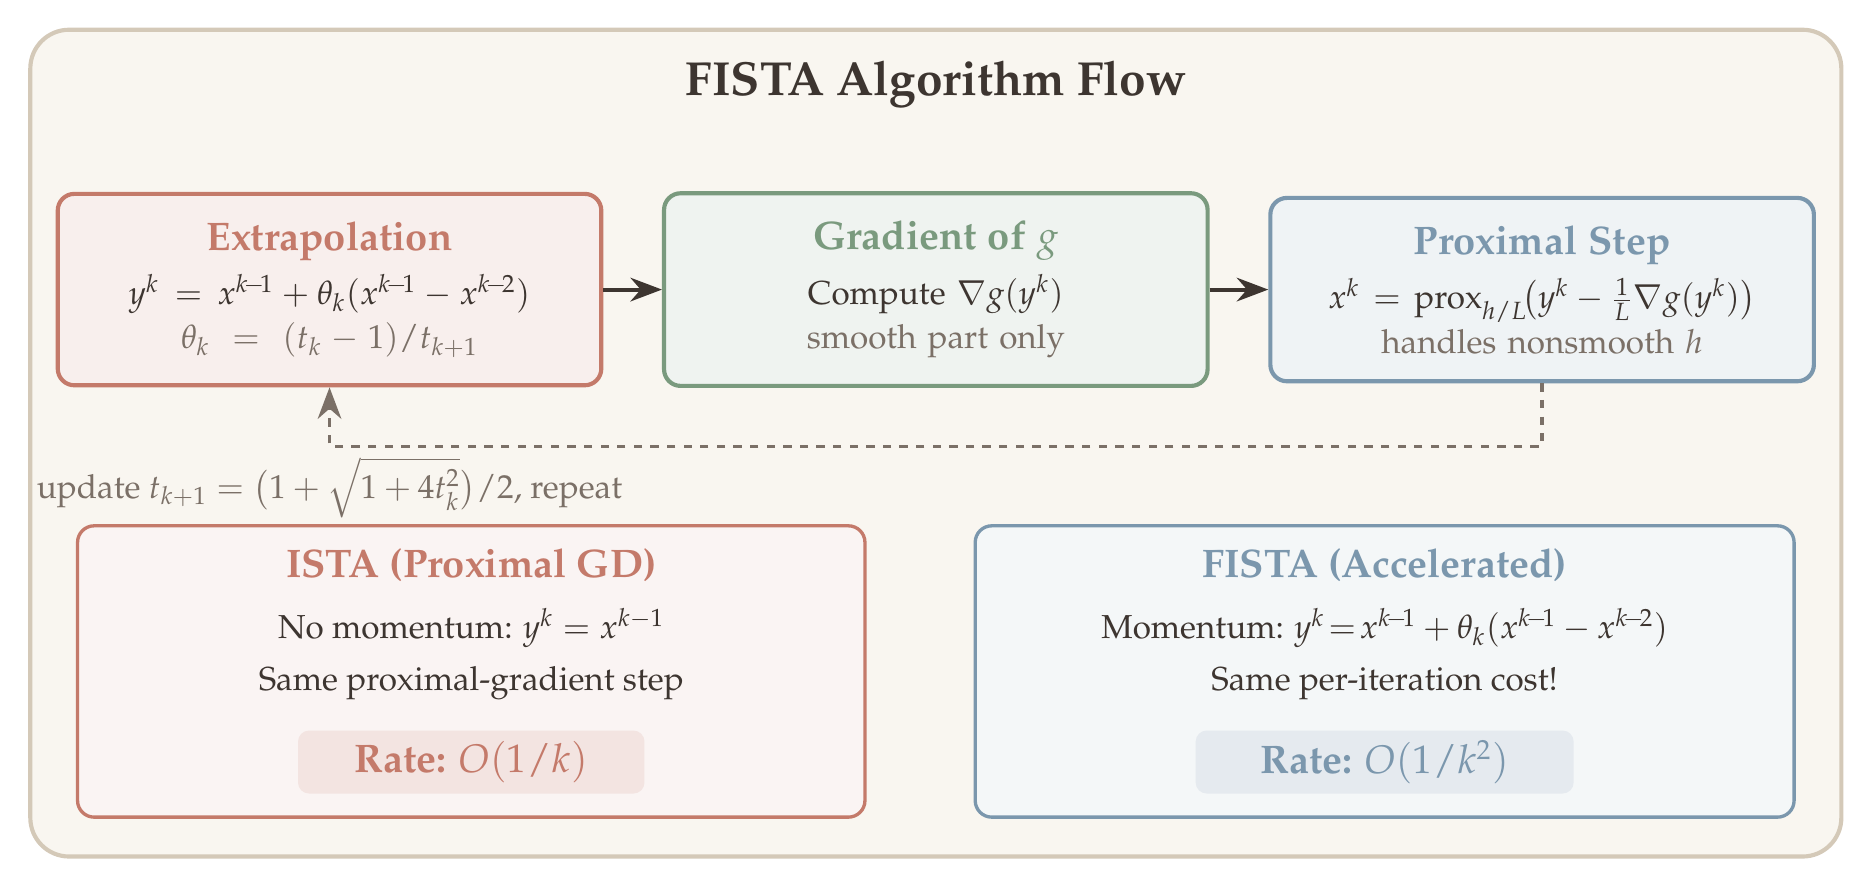
\begin{tikzpicture}[
  >={Stealth[length=4mm, width=3mm]},
  every node/.style={text=dkbrown, font=\large},
  box/.style={rounded corners=6pt, line width=1.5pt, minimum height=2.2cm, text width=6.2cm, align=center, inner sep=10pt},
]

% Background
\fill[cream, rounded corners=14pt] (0,0) rectangle (23,10.5);
\draw[border, line width=1.5pt, rounded corners=14pt] (0,0) rectangle (23,10.5);

% Title
\node[font=\LARGE\bfseries, text=dkbrown] at (11.5,9.8) {FISTA Algorithm Flow};

% Step 1: Extrapolation
\node[box, fill=terracotta!12, draw=terracotta] (ext) at (3.8,7.2) {%
  {\Large\bfseries\color{terracotta}Extrapolation}\\[4pt]
  $y^k = x^{k\!-\!1} + \theta_k(x^{k\!-\!1} - x^{k\!-\!2})$\\[2pt]
  {\color{wmgray}$\theta_k = (t_k - 1)/t_{k+1}$}
};

% Step 2: Gradient of g
\node[box, fill=sage!12, draw=sage] (grad) at (11.5,7.2) {%
  {\Large\bfseries\color{sage}Gradient of $g$}\\[4pt]
  Compute $\nabla g(y^k)$\\[2pt]
  {\color{wmgray}smooth part only}
};

% Step 3: Proximal step
\node[box, fill=stblue!12, draw=stblue] (prox) at (19.2,7.2) {%
  {\Large\bfseries\color{stblue}Proximal Step}\\[4pt]
  $x^k = \mathrm{prox}_{h/L}\!\bigl(y^k - \tfrac{1}{L}\nabla g(y^k)\bigr)$\\[2pt]
  {\color{wmgray}handles nonsmooth $h$}
};

% Arrows between steps
\draw[dkbrown, line width=1.5pt, ->] (ext.east) -- (grad.west);
\draw[dkbrown, line width=1.5pt, ->] (grad.east) -- (prox.west);

% Feedback loop
\draw[wmgray, line width=1.2pt, dashed, ->]
  (prox.south) -- ++(0,-0.8) -| (ext.south)
  node[pos=0.5, below, font=\large, text=wmgray] {%
    update $t_{k+1} = \bigl(1 + \sqrt{1 + 4t_k^2}\bigr)/2$, repeat};

% --- Comparison boxes ---
% ISTA box
\draw[terracotta, line width=1.2pt, rounded corners=6pt, fill=terracotta!8]
  (0.6,0.5) rectangle (10.6,4.2);
\node[font=\Large\bfseries, text=terracotta] at (5.6,3.7) {ISTA (Proximal GD)};
\node[font=\large] at (5.6,2.9) {No momentum: $y^k = x^{k-1}$};
\node[font=\large] at (5.6,2.2) {Same proximal-gradient step};
\fill[terracotta!20, rounded corners=4pt] (3.4,0.8) rectangle (7.8,1.6);
\node[font=\Large\bfseries, text=terracotta] at (5.6,1.2) {Rate: $O(1/k)$};

% FISTA box
\draw[stblue, line width=1.2pt, rounded corners=6pt, fill=stblue!8]
  (12.0,0.5) rectangle (22.4,4.2);
\node[font=\Large\bfseries, text=stblue] at (17.2,3.7) {FISTA (Accelerated)};
\node[font=\large] at (17.2,2.9) {Momentum: $y^k\!=\!x^{k\!-\!1} + \theta_k(x^{k\!-\!1} - x^{k\!-\!2})$};
\node[font=\large] at (17.2,2.2) {Same per-iteration cost!};
\fill[stblue!20, rounded corners=4pt] (14.8,0.8) rectangle (19.6,1.6);
\node[font=\Large\bfseries, text=stblue] at (17.2,1.2) {Rate: $O(1/k^2)$};

\end{tikzpicture}
\end{document}
